\chapter{Final Evaluation}
\label{chap:evaluation}
\centerline{\rule{149mm}{.02in}}
\vspace{2cm}

We have shown that the point $kd$-tree greatly outperforms the Pyramid tree for the two scientific datasets. For all synthetic data and the 3D point cloud dataset, the Pyramid tree is faster, especially with regard to point deletion.

This chapter will explore the reasons for this, determining what characteristics the astrophysics dataset cause the performance of the structures to degenerate. The chapter will conclude by discussing the types of data suitable for the Pyramid Tree and $kd$-Tree, along with some further discussion on the implications of the results from this evaluation.

\section{Characteristics of Astrophysics Dataset}
\label{sec:data-characteristics}

\begin{figure}
	\begin{center}
		\begin{subfloat}[Uniform\label{fig:uniform-freq-distribution}]{%
			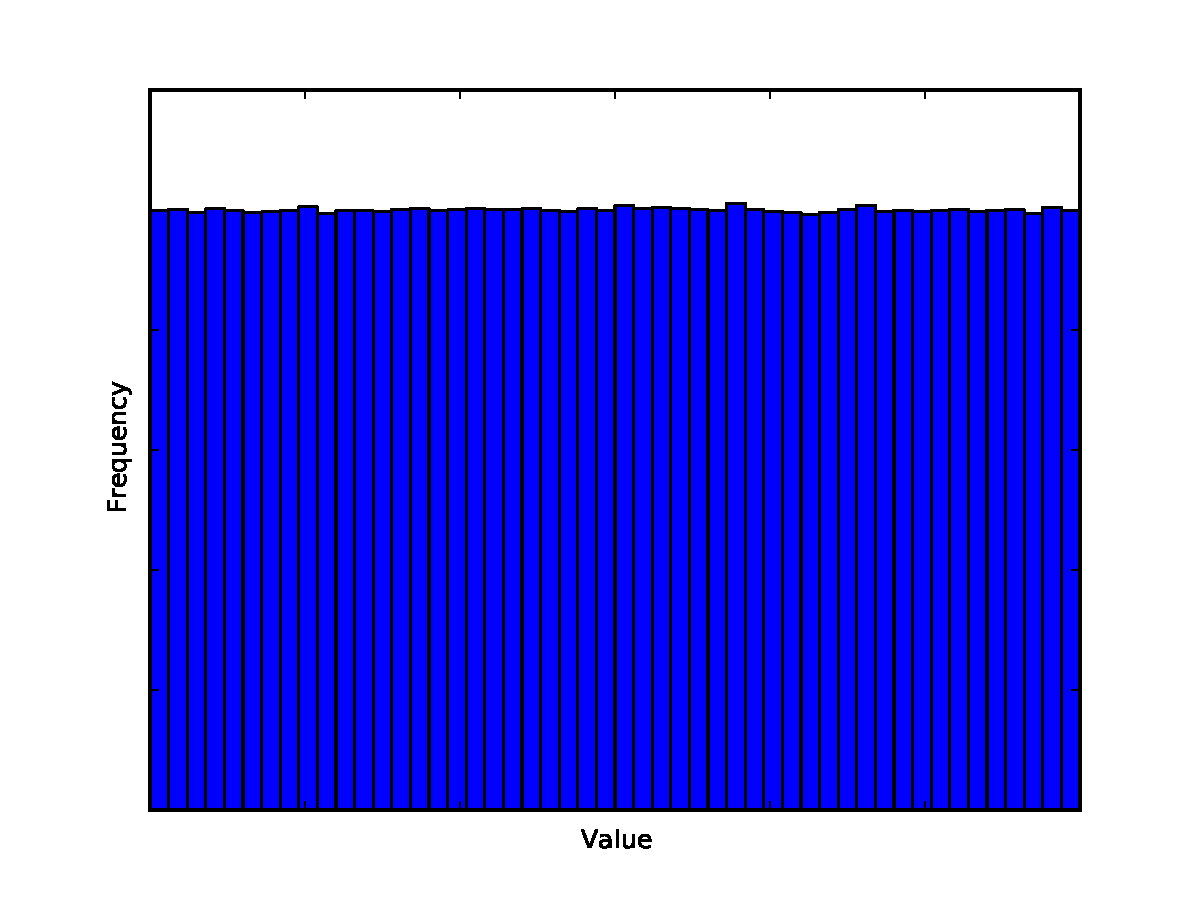
\includegraphics[scale=0.2]{figures/freqdist_uniform.pdf}
		}
		\end{subfloat}~
		\begin{subfloat}[Gaussian\label{fig:gaussian-freq-distribution}]{%
			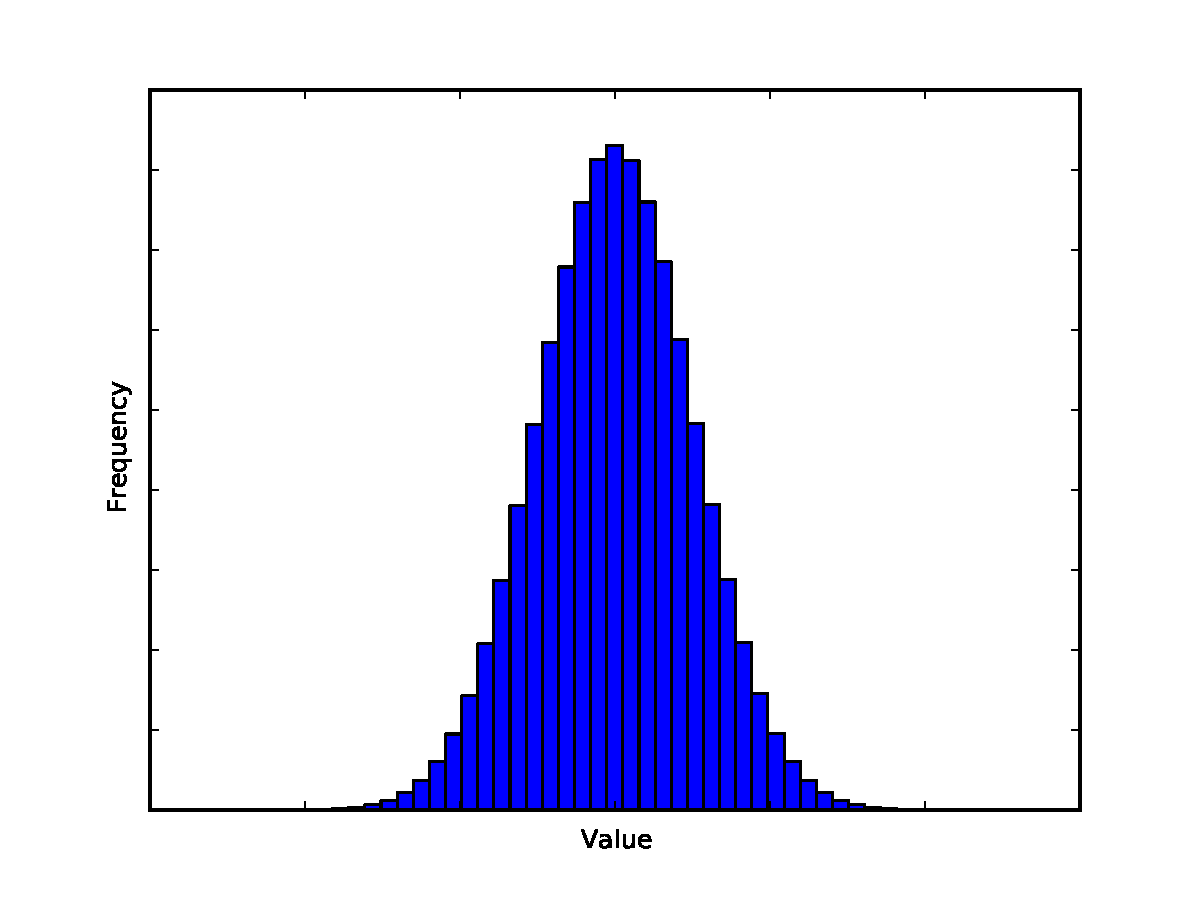
\includegraphics[scale=0.2]{figures/freqdist_gaussian.pdf}
		}
		\end{subfloat}~
		\begin{subfloat}[Gamma (Skewed)\label{fig:skewed-freq-distribution}] {%
			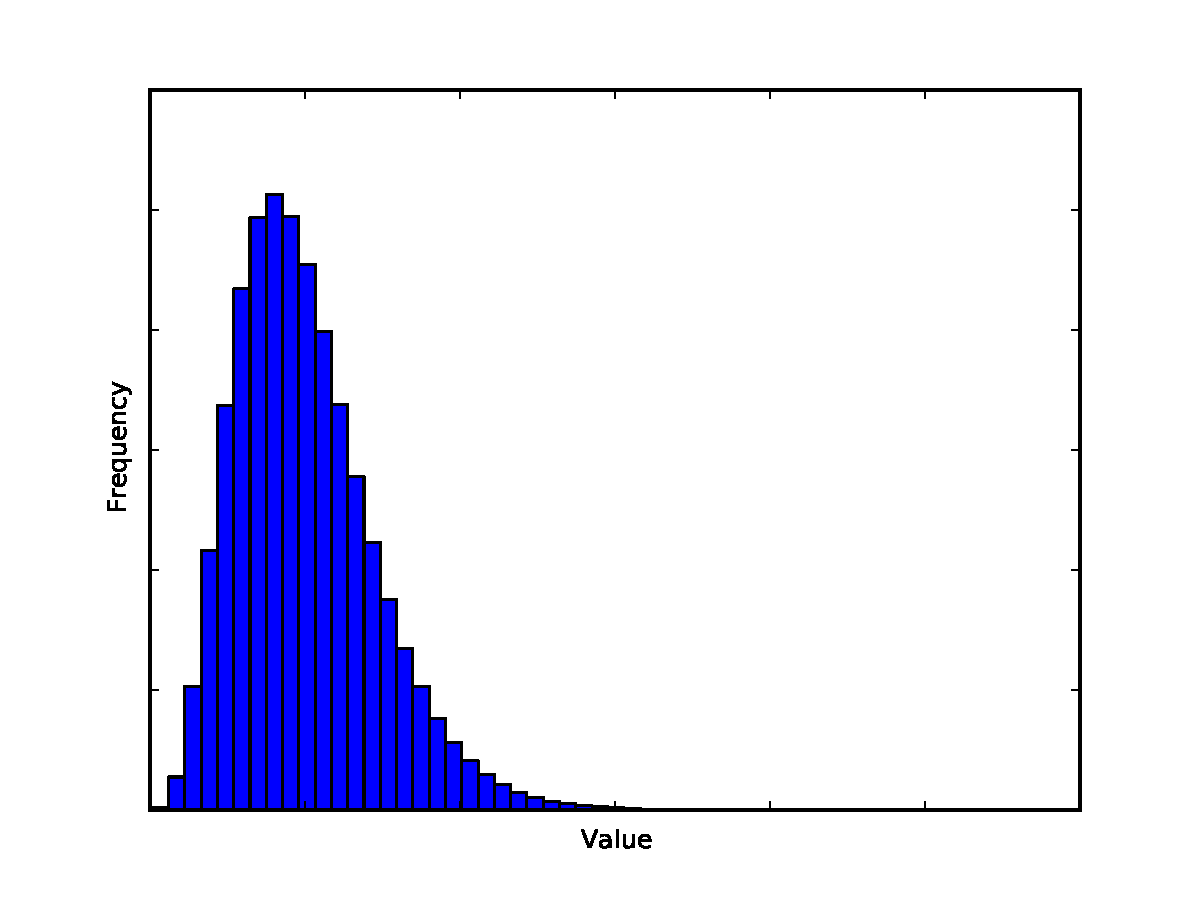
\includegraphics[scale=0.2]{figures/freqdist_gamma.pdf}
		}
		\end{subfloat}
	\end{center}

	\caption{Three Types of Frequency Distributions}
	\label{fig:frequency-distributions}
\end{figure}

A dataset is considered \textit{skewed} if a greater number of points are present in certain regions of the data space than other regions of the space. That is, the underlying frequency or probability distribution of point locations is non-uniform. Figure \ref{fig:frequency-distributions} visualises uniform, Gaussian and skewed frequency distributions using histograms. Intuitively, the skewness of a dataset increases as the \textit{difference} between the frequency/probability of points in different spatial regions increases.

Histograms are used to visualise the frequency distributions of one-dimensional data. Since this project deals with multi-dimensional data, multiple histograms, one for each dimension, can be produced to gain insight into point distribution. The astrophysics dataset was computed using a 3D sampling lattice, computing ten fields at each point. The original simulation imposes uses interpolation between points in the sampling lattice \cite{astrophysics-dataset}. Carr et al. discusses how this interpolation ``implicitly applies the spatial relation between sample points" and shows that histograms are equivalent to nearest-neighbour interpolation. This means histograms poorly represent datasets that use higher-order interpolants, such as the astrophysics dataset, because it ``over-emphasizes densely-sampled regions and under-emphasizes sparsely-sampled regions". 

Isosurface statistics have been proposed as a superior representation of datasets \cite{histograms-and-isosurfaces}. They are conceptually and computationally more complex to compute however. Due to project time constraints, isosurface statistics shall not be used. While histograms are poorer representation of the data, the aim of this evaluation is determine the magnitude of the skew present in the different dimensions of the dataset. Histograms still provide a visual representation of data distribution, even if it is not as accurate as desired. Therefore, histograms will be used to visualise the distribution of the astrophysics dataset.

\begin{figure}
	\begin{center}
		\begin{subfloat}[Dimension 1 (total particle density)]{%
			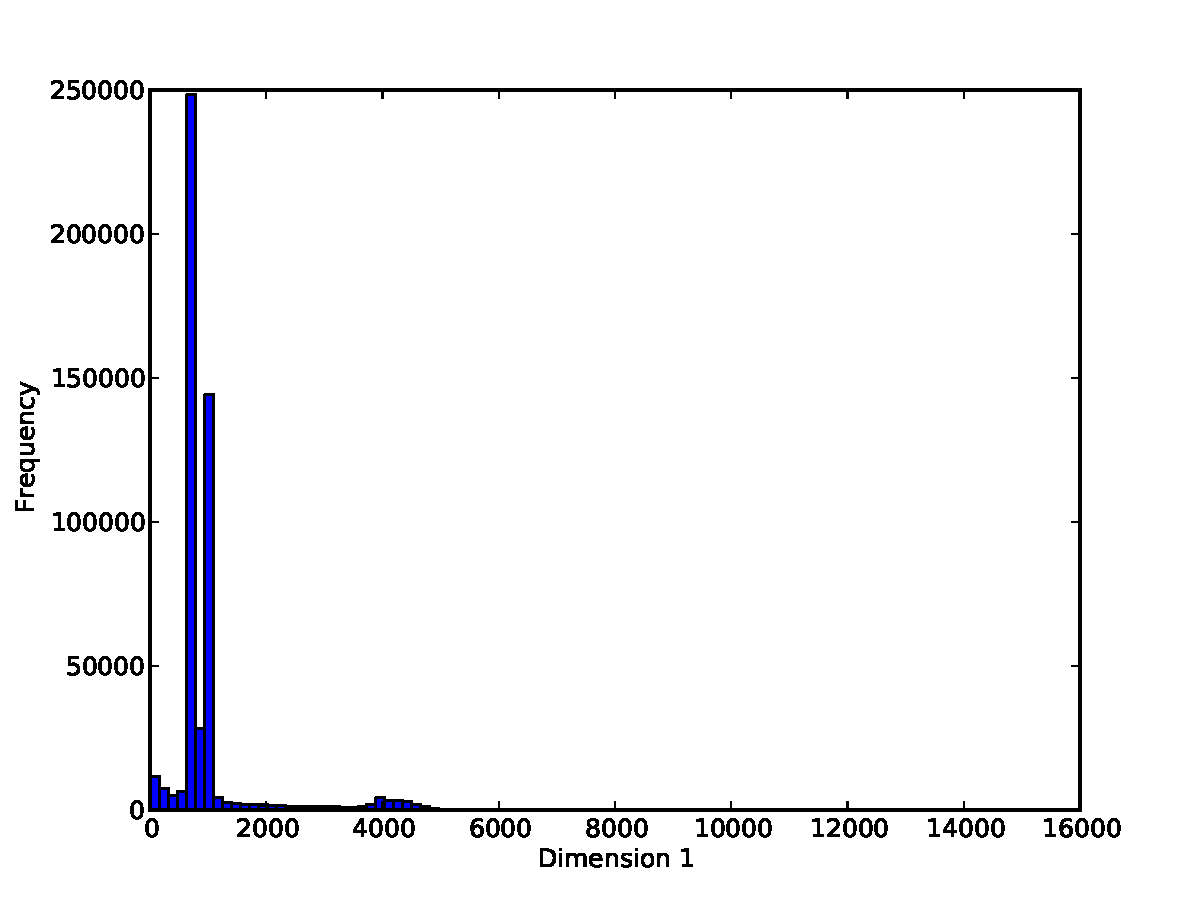
\includegraphics[scale=0.36]{figures/histograms/astrophysics_500000_0.pdf}
		}
		\end{subfloat}~
		\begin{subfloat}[Dimension 2 (gas temperature)]{%
			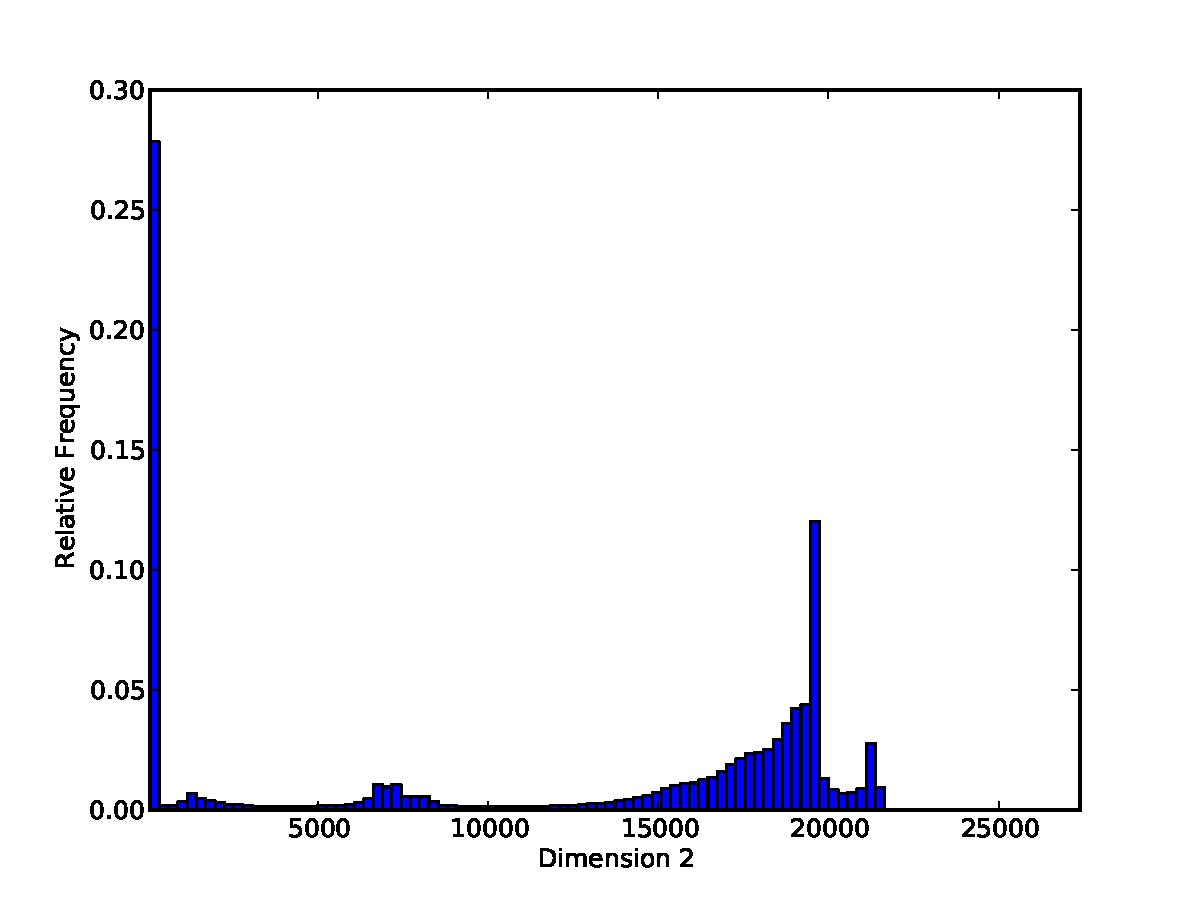
\includegraphics[scale=0.36]{figures/histograms/astrophysics_500000_1.pdf}
		}
		\end{subfloat}
	\end{center}

	\caption{Frequency Distributions of Dimensions 1 and 2 of Astrophysics Dataset}
	\label{fig:astrophysics-histograms1}
\end{figure}

\begin{figure}
	\begin{center}
		\begin{subfloat}[Dimension 3 (H mass abundance)]{%
			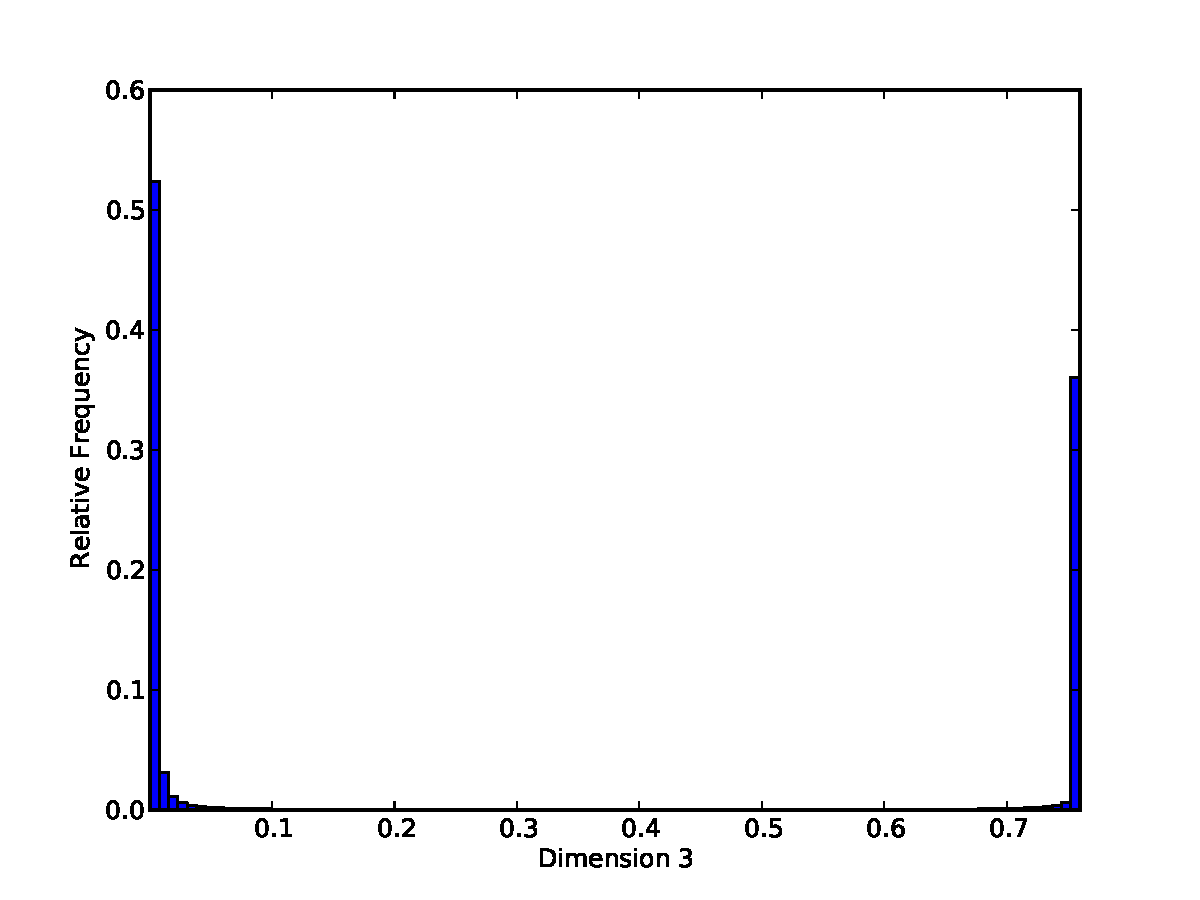
\includegraphics[scale=0.36]{figures/histograms/astrophysics_500000_2.pdf}
		}
		\end{subfloat}~
		\begin{subfloat}[Dimension 7 (He${}^{++}$ mass abundance)]{%
			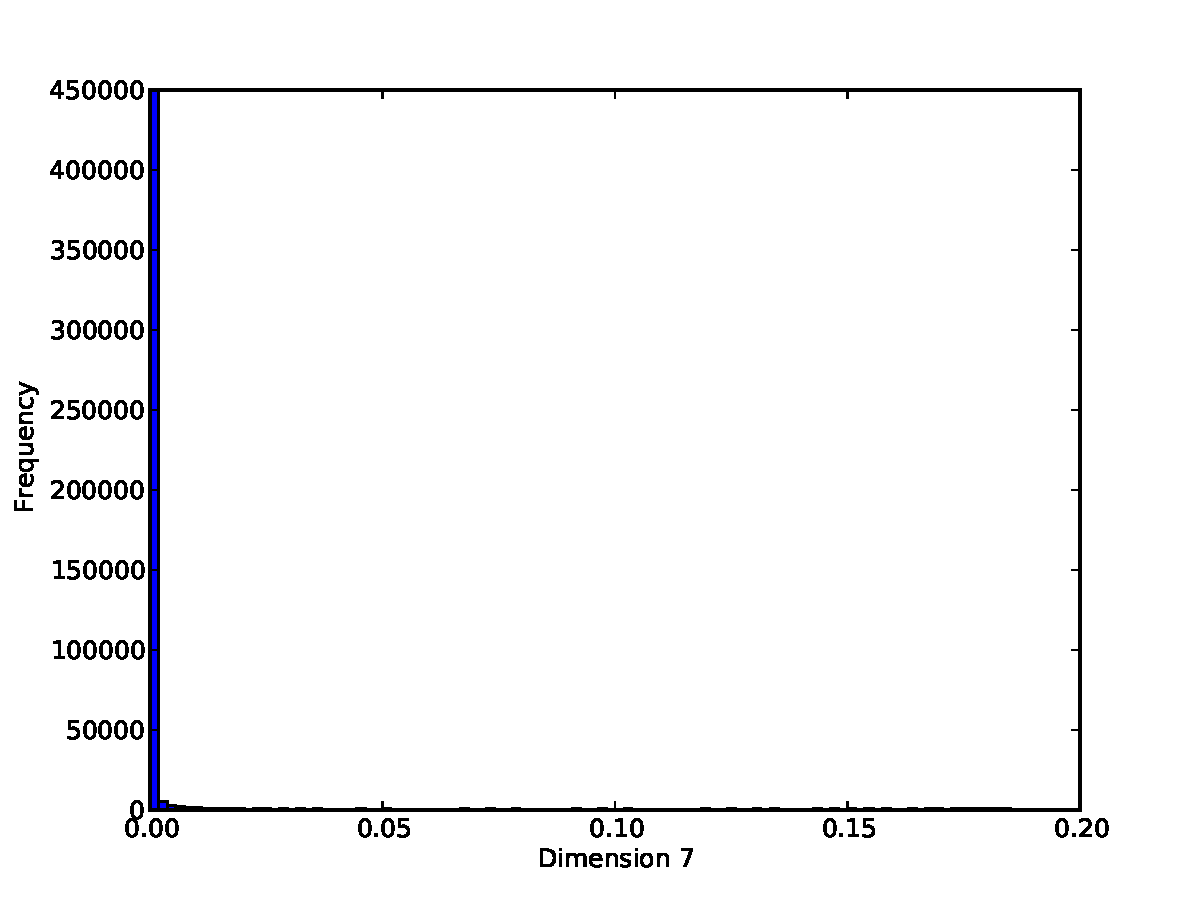
\includegraphics[scale=0.36]{figures/histograms/astrophysics_500000_6.pdf}
		}
		\end{subfloat}
	\end{center}

	\caption{Frequency Distributions of Dimensions 3 and 7 of Astrophysics Dataset}
	\label{fig:astrophysics-histograms2}
\end{figure}

Ten histograms have been generated using each dimension of the sampled astrophysics dataset used for performance analyses in Chapter \ref{chap:design-and-implementation}.Figures \ref{fig:astrophysics-histograms1} and \ref{fig:astrophysics-histograms2} show histograms of dimensions 1, 2, 3 and 7. The histograms for the remaining dimensions are provided in Appendix \ref{sec:app-histograms} since they have distributions similar to the dimensions shown here and thus, add little information. Using these histograms, the following observations can be made:
\begin{enumerate}
	\item the first two dimensions, total particle density and gas temperature, appear to have the greatest variance, although there are still very large peaks
	\item the majority of points are clustered on the lower or upper boundaries of dimensions 3, 4, 5 and 6. The respective histograms have massive peaks at either end of the distribution and much smaller peaks in-between
	\item the majority of the points are clustered on the lower boundary of dimensions 7, 8, 9 and 10 (single large peak at lower boundary)
\end{enumerate}
The astrophysics dataset is therefore highly skewed, since most points are clustered at the boundaries of the dimensions. It follows that the vast majority of the data space has little to no points, making the dataset \textit{sparse}.

\section{Effect of Distribution on Pyramid Tree}

We now explore the effect of the highly skewed distribution on the Pyramid Tree. Recall that the Pyramid Tree maps a point $v$ to a single scalar named the Pyramid value $pv_v$. Figure \ref{fig:astrophysics-pyval-histogram1} illustrates the distribution of Pyramid values within the sampled astrophysics dataset using a histogram. Ideally, the distribution of Pyramid values should be uniform, since this will minimise average bucket size which, as shown in Section \ref{sec:iteration2}, is the main factor which affects the Pyramid Tree's performance.

Figure \ref{fig:astrophysics-pyval-histogram1} shows a massively skewed distribution, with the majority of Pyramid values lying in the same region. This increases the likelihood that points will be mapped to the same buckets, increasing average bucket size. Figures \ref{fig:astrophysics-pyval-histogram2} and \ref{fig:astrophysics-pyval-histogram3} show pyramid value distribution when just using dimensions 1 and 2, and 3 and 7, respectively. Notice how pyramid value distribution is considerably more skewed when using the first dimensions 3 and 7 compared to the first two dimensions. TODO

TODO: boundary ignore

\begin{figure}
	\begin{center}
		\begin{subfloat}[All Dimensions\label{fig:astrophysics-pyval-histogram1}]{%
			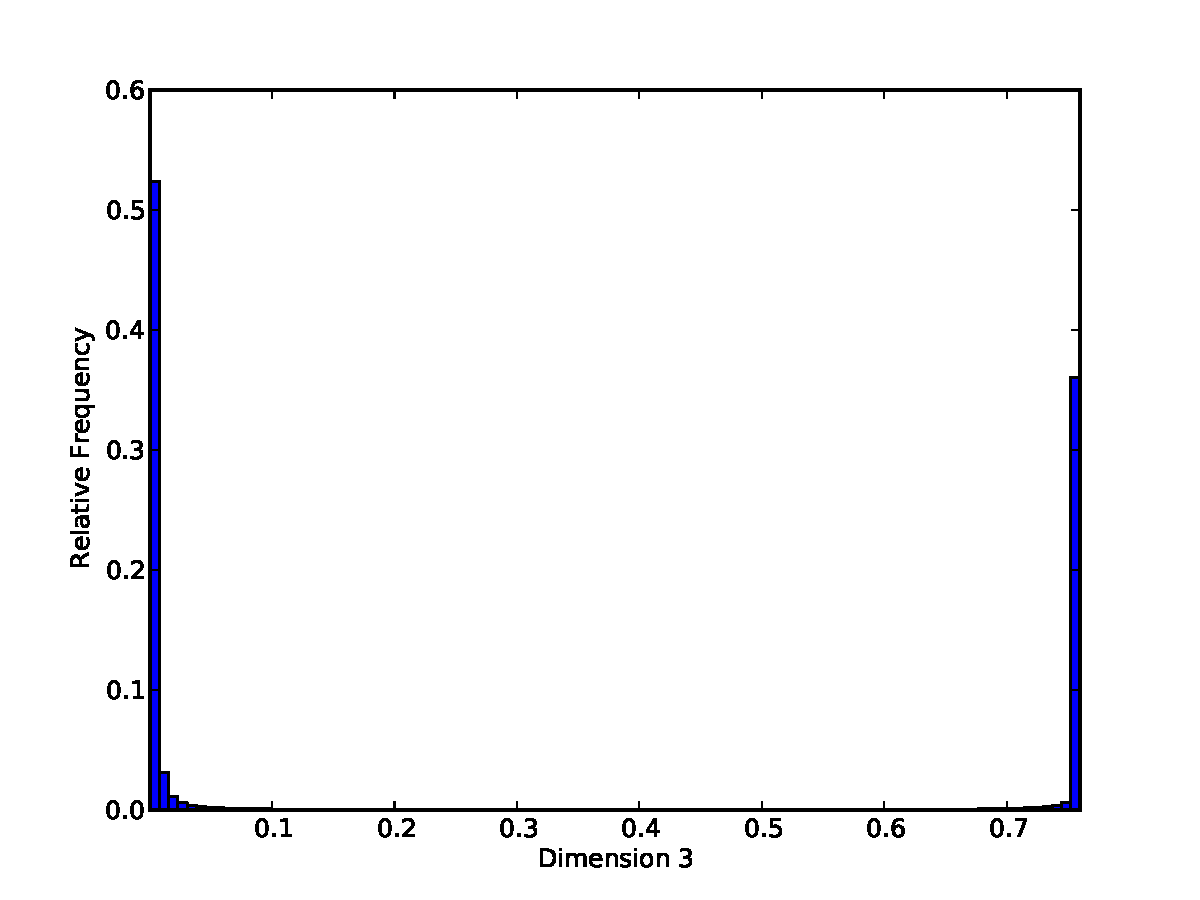
\includegraphics[scale=0.25]{figures/histograms/astrophysics_500000_2.pdf}
		}
		\end{subfloat}~
		\begin{subfloat}[Dimensions 1 and 2 \label{fig:astrophysics-pyval-histogram2}]{%
			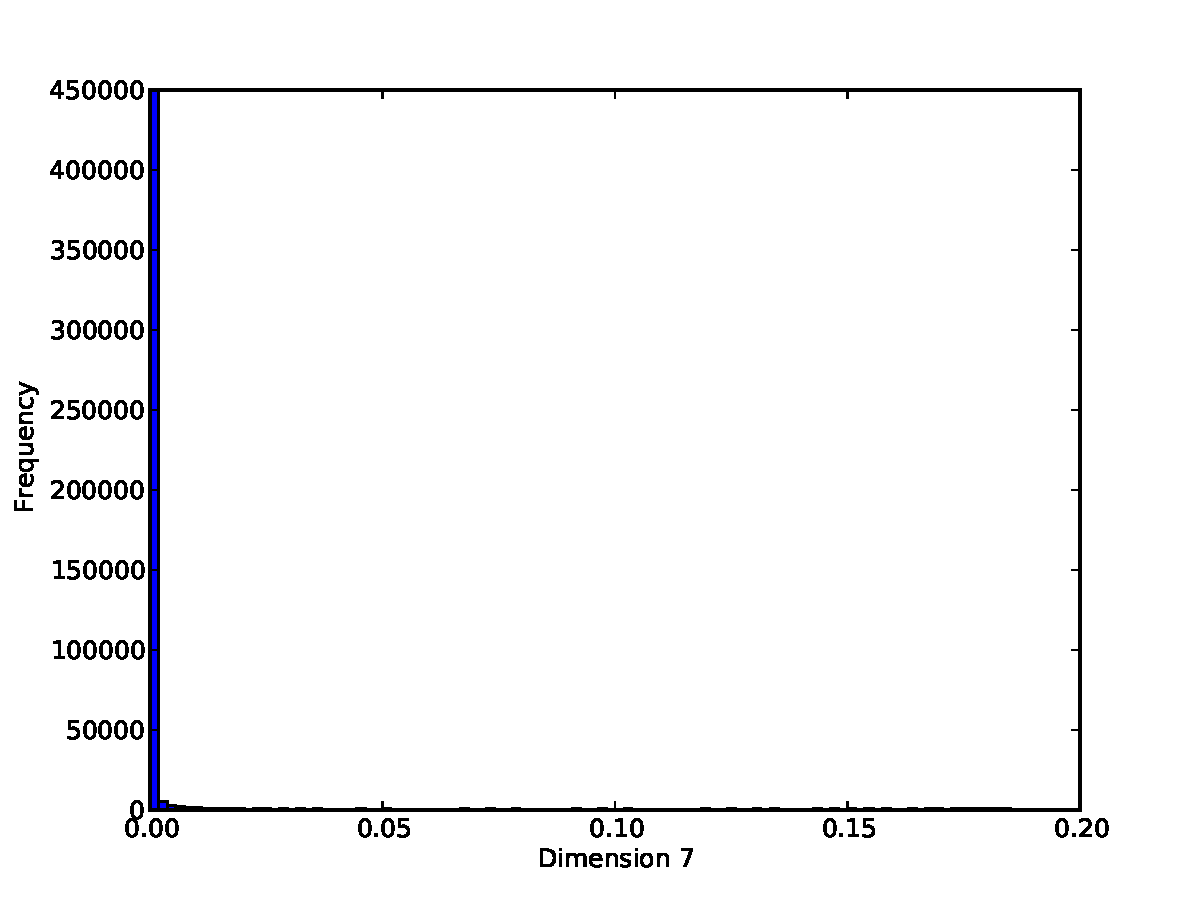
\includegraphics[scale=0.25]{figures/histograms/astrophysics_500000_6.pdf}
		}
		\end{subfloat}
		\begin{subfloat}[Dimensions 3 and 7\label{fig:astrophysics-pyval-histogram3}]{%
			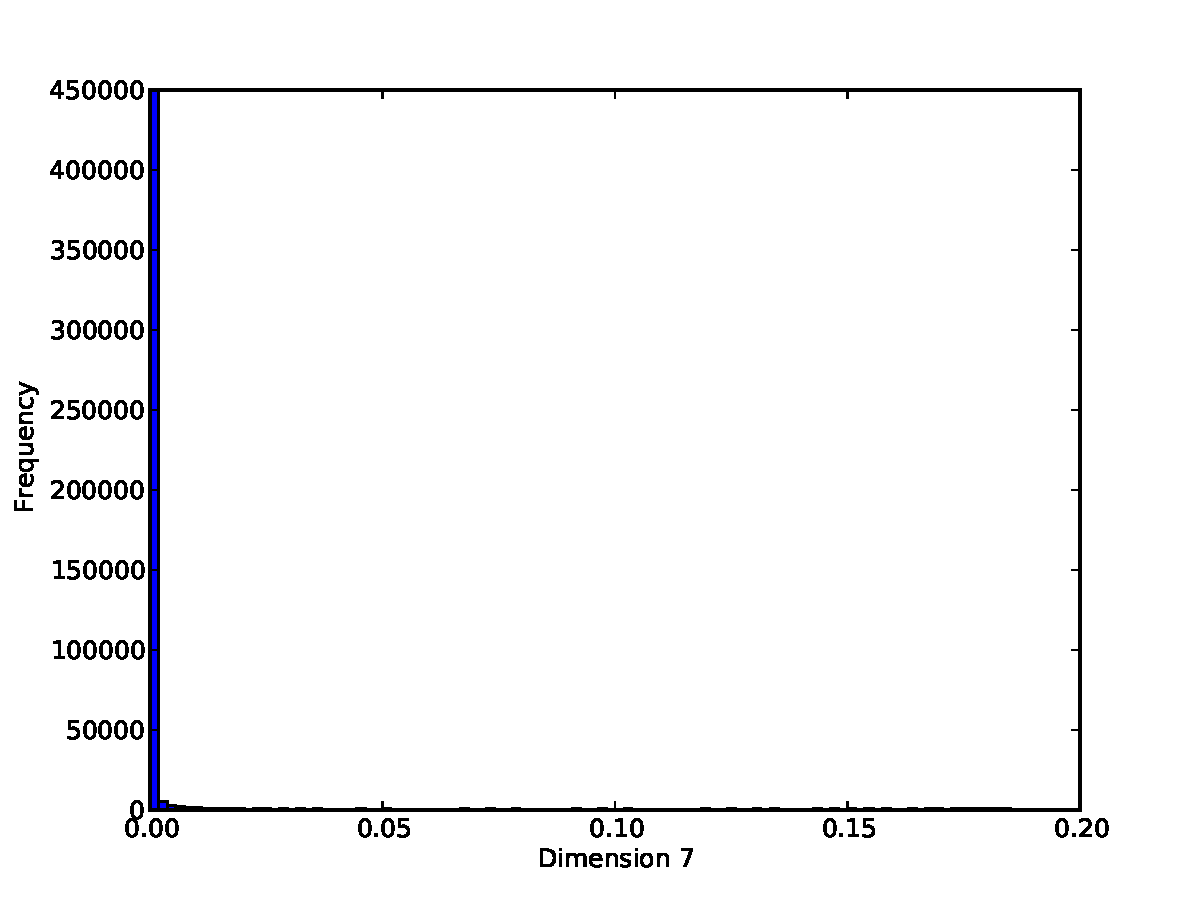
\includegraphics[scale=0.25]{figures/histograms/astrophysics_500000_6.pdf}
		}
		\end{subfloat}
		\begin{subfloat}[Ignoring Boundary Values\label{fig:astrophysics-pyval-histogram4}]{%
			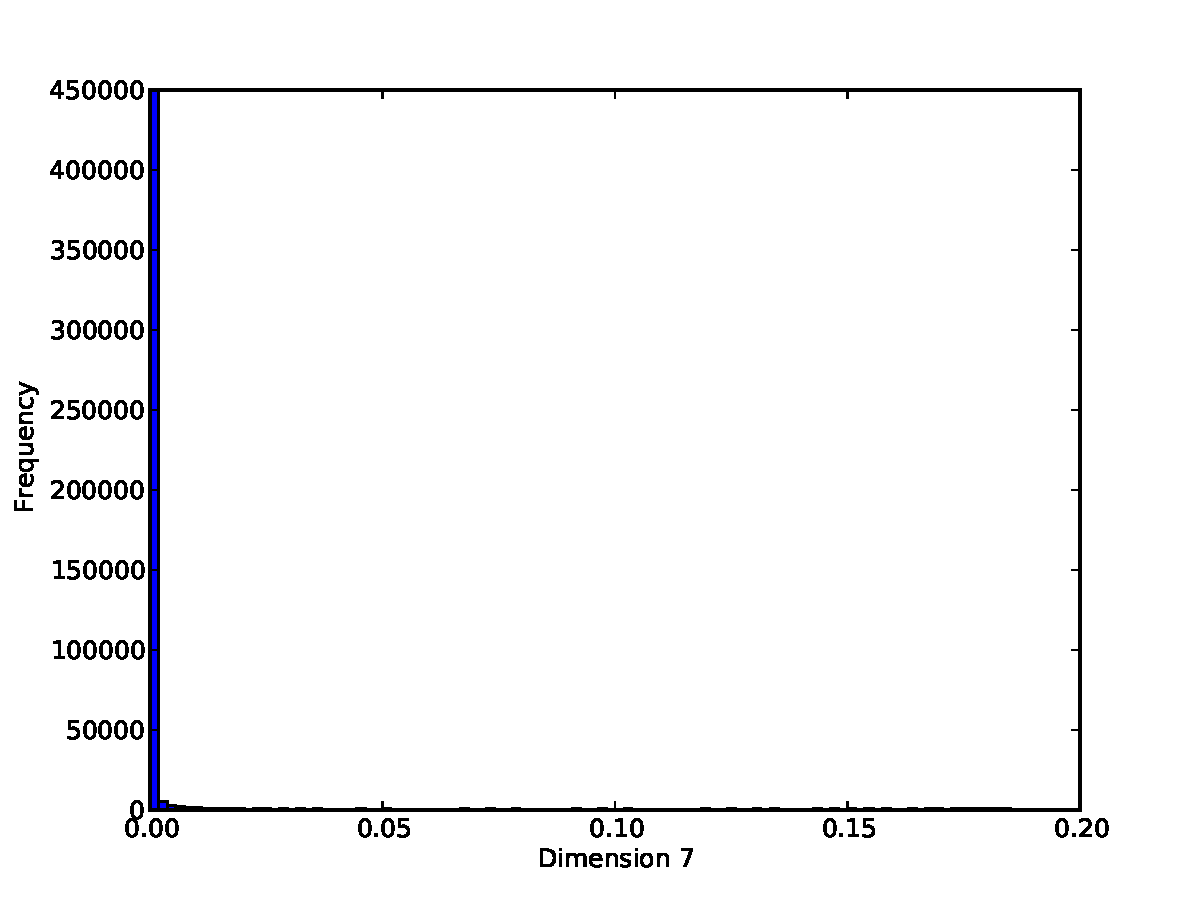
\includegraphics[scale=0.25]{figures/histograms/astrophysics_500000_6.pdf}
		}
		\end{subfloat}
	\end{center}

	\caption{Distribution of Pyramid Values in Different Samples of Astrophysics Dataset}
	\label{fig:astrophysics-pyval-histograms}
\end{figure}


\section{Effect of Distribution on $kd$-Tree}

TODO

\section{Why So Sparse?}

TODO: conjecture on why the astrophysics dataset is so sparse -- referencing literature and how this might support stuff

\section{Suitable Data for Index Structures}

TODO